\chapter{Introduction}

%\begin{center}
%  {\it ``If could add an introductionary text here.''}
%  \vspace{1cm}
%\end{center}

Our Universe is well described by the $\lambda$CDM %by the Big Bang 
model. In this model the universe is composed by baryonic matter, dark matter and dark energy. We can only observe the baryonic matter in the Universe, which makes up only $\sim 5\%$ of its content, while dark matter is $\sim 27\%$ and dark energy $\sim 68\%$. In this model the chemical composition of the Universe determined by the cosmological nucleosynthesis which takes place in the first minutes of its life, and is mostly of hydrogen and helium (gas) and very few heavier elements (\emph{metals}). As the universe expands in time, dark matter falls into the potential wells arisen from the cosmic fluctuations, thereby dragging baryonic matter along with it. Dark matter will collapse to form halos, while baryonic matter will collapse to form stars and galaxies \citep{2009ApJS..180..330K,2007ApJS..170..377S,2020A&A...641A...1P}. It is commonly believed that in the center of each galaxy lies a supermassive black hole (SMBH, or simply BH), an object whose density is so high that not even light can escape it. 

While it is easy to describe the behavior of dark matter, as it only interacts gravitationally, the same cannot be said of baryonic physics, which rules galaxy evolution. As the stars evolve they produce more and more metals, giving rise to dust and creating older stellar populations. Stars interact with their environment through strong stellar winds and can explode as supernovae. More gas supplies can flow into the galaxy from the intergalactic medium, the gas can cool down to form new stars, but also fall into the central potential well of the galaxy to feed the SMBH. The galaxy itself can undergo morphological evolution as it interacts with its environment and/or through mergers with other galaxies. 

In this thesis we are going to study the evolution of the gas accretion by tracing the growth of BH, i.e. the black hole accretion rate (BHAR), and the accretion of new stellar populations, measured as the star formation rate (SFR) as a function of time and of the life phase of the galaxy, defined by how actively it is forming new stars.
%When the star formation rate (SFR) and the central super-massive black hole accretion rate (BHAR) of a galaxy reach appreciable values, they enter the regime of the so called ``active galaxies''.

The rapid accretion of the SMBH in the core of the galactic center, that defines an active galactic nucleus (AGN), is usually observable at various wavelengths, since it involves, directly or indirectly, a large number of physical mechanisms. Nowadays, the differences among AGN showing different observational characteristics are explained in the context of the unified model \citep{1977ApJ...213..635R, 1984ApJ...278..499A, 1985ApJ...297..621A, 1993ARA&A..31..473A, 1995PASP..107..803U, 2015ARA&A..53..365N}, as due to the orientation with respect to the observer.

As already mentioned, galaxies interact with their medium. They can undergo violent interactions or mergers that can end up causing a morphological change or they can evolve in a more passive sort of way in which they consume the gas that is already present in situ and may receive a slow gas inflow from the cosmic web of filaments containing pristine gas. The latter case is what we call secular evolution and in this case, the SFR of a galaxy
%During the secular evolution of a galaxy, its SFR 
seems to be regulated by a simple empirical relation: the bigger the galaxy is, in terms of stellar mass M$_*$, the higher the SFR is. This law, usually referred to as main sequence (MS) of star-forming galaxies \citep{2004MNRAS.351.1151B, 2007A&A...468...33E, 2007ApJ...670..156D, 2007ApJ...660L..47N, 2014MNRAS.443...19R, 2017MNRAS.465.3390A}, seems to be valid for local as well as for distant galaxies, for a wide range of stellar masses, and considering different SFR tracers. A galaxy can be considered as ``active'' by the point of view of the star formation, when its SFR is consistent or higher than the main sequence. A galaxy is then ``passive'' (or equivalently ``quiescent'') when the SFR is very low or absent. At the opposite side of the main sequence, a special class of star forming galaxies is represented by the so called ``starbursts'', which show SFRs even ten times, or higher than that of the main sequence. These rare objects, represent a very peculiar and still not well known phase of galaxy evolution. 

\section{SFR and its tracers}% Da Ivano e da http://ned.ipac.caltech.edu/level5/Sept12/Calzetti/Calzetti1_2.html
%Párrafo introductivo sobre M*, SFR...

There are many ways in which the SFR can be inferred from the integrated light emitted by a galaxy. Calibrations of SFR indicators have been presented in the literature for almost 30 years, derived across the full electromagnetic spectrum, from the X-ray, through the ultraviolet (UV), via the optical and infrared (IR), all the way to the radio, and using both continuum and line emission. Extensive reviews of this topic are reported in, e.g., \citet{1998ARA&A..36..189K,2012ARA&A..50..531K,2012MNRAS.420.2190V}. The basic goal is to identify emission that probes newly or recently formed stars, while avoiding as much as possible contributions from evolved stellar populations.

In unresolved systems, SFR indicators are merely measures of luminosity, either monochromatic or integrated over some wavelength range, with the goal of targeting continuum or line emission that is sensitive to the short-lived massive stars. The conversion from the luminosity of massive stars to a SFR is performed under the assumption that: (1) the star formation has been roughly constant over the time-scale probed by the specific emission being used; (2) the stellar initial mass function (IMF) is known (or is a controllable parameter) so that the number of massive stars can be extrapolated to the total number of high$+$low mass stars formed; and (3) the stellar IMF is fully sampled, meaning that at least one star is formed in the highest-mass bin, and all other mass bins are populated accordingly with one or more stars.

SFR indicators in the UV/optical/near-IR range ($\sim$0.1--5~\textmu m) probe the direct stellar light emerging from galaxies, while SFR indicators in the mid/far-IR ($\sim$5--1000~\textmu m) probe the stellar light reprocessed by dust. In addition to direct or indirect stellar emission, the ionizing photon rate, as traced by the gas ionized by massive stars, can be used to define SFR indicators; photo-ionized gas usually dominates over shock-ionized gas in galaxies or large structures within galaxies \citep[e.g.,][]{2004AJ....127.1405C,2011ApJ...731...45H}. Tracers include hydrogen recombination lines, from the optical, through the near-IR, all the way to radio wavelengths, forbidden metal lines, and, in the millimeter range, the free-free (Bremsstrahlung) emission. The X-ray emission produced by high-mass X-ray binaries, massive stars, and supernovae can also be used to trace SFRs \citep{2017MNRAS.465.3390A}. Finally, the synchrotron emission from galaxies can be calibrated as a SFR indicator \citep{1992ARA&A..30..575C}, since cosmic rays are produced and accelerated in supernova remnants, and core-collapse supernovae represent 70\% or more of the total supernovae in star-forming galaxies \citep{2009A&A...503..137B}.

\section{AGN and their emission mechanisms}
Active galactic nuclei are the ensemble of physical and observational phenomena that occur at the very center of galaxies and ascribable to the presence of a SMBH accreting matter at high rates. As can be seen in Fig.~\ref{fig:AGN_SED}, their emission encompasses the whole electromagnetic spectrum and cannot be explained by stars, gas and dust alone%, the presence of a SMBH is therefore required
. Luminosity variability measurements allow to determine the size of these sources that are not bigger than few parsecs. AGN are the most powerful emitting sources in the universe and for quite a long time, they were the only kind of source that was detectable at high redshifts. Nowadays, they represent one of the important mechanisms, together with the SF, that seem to drive the evolution of galaxies and the environment in which they evolve.

\begin{figure}
\begin{center}
  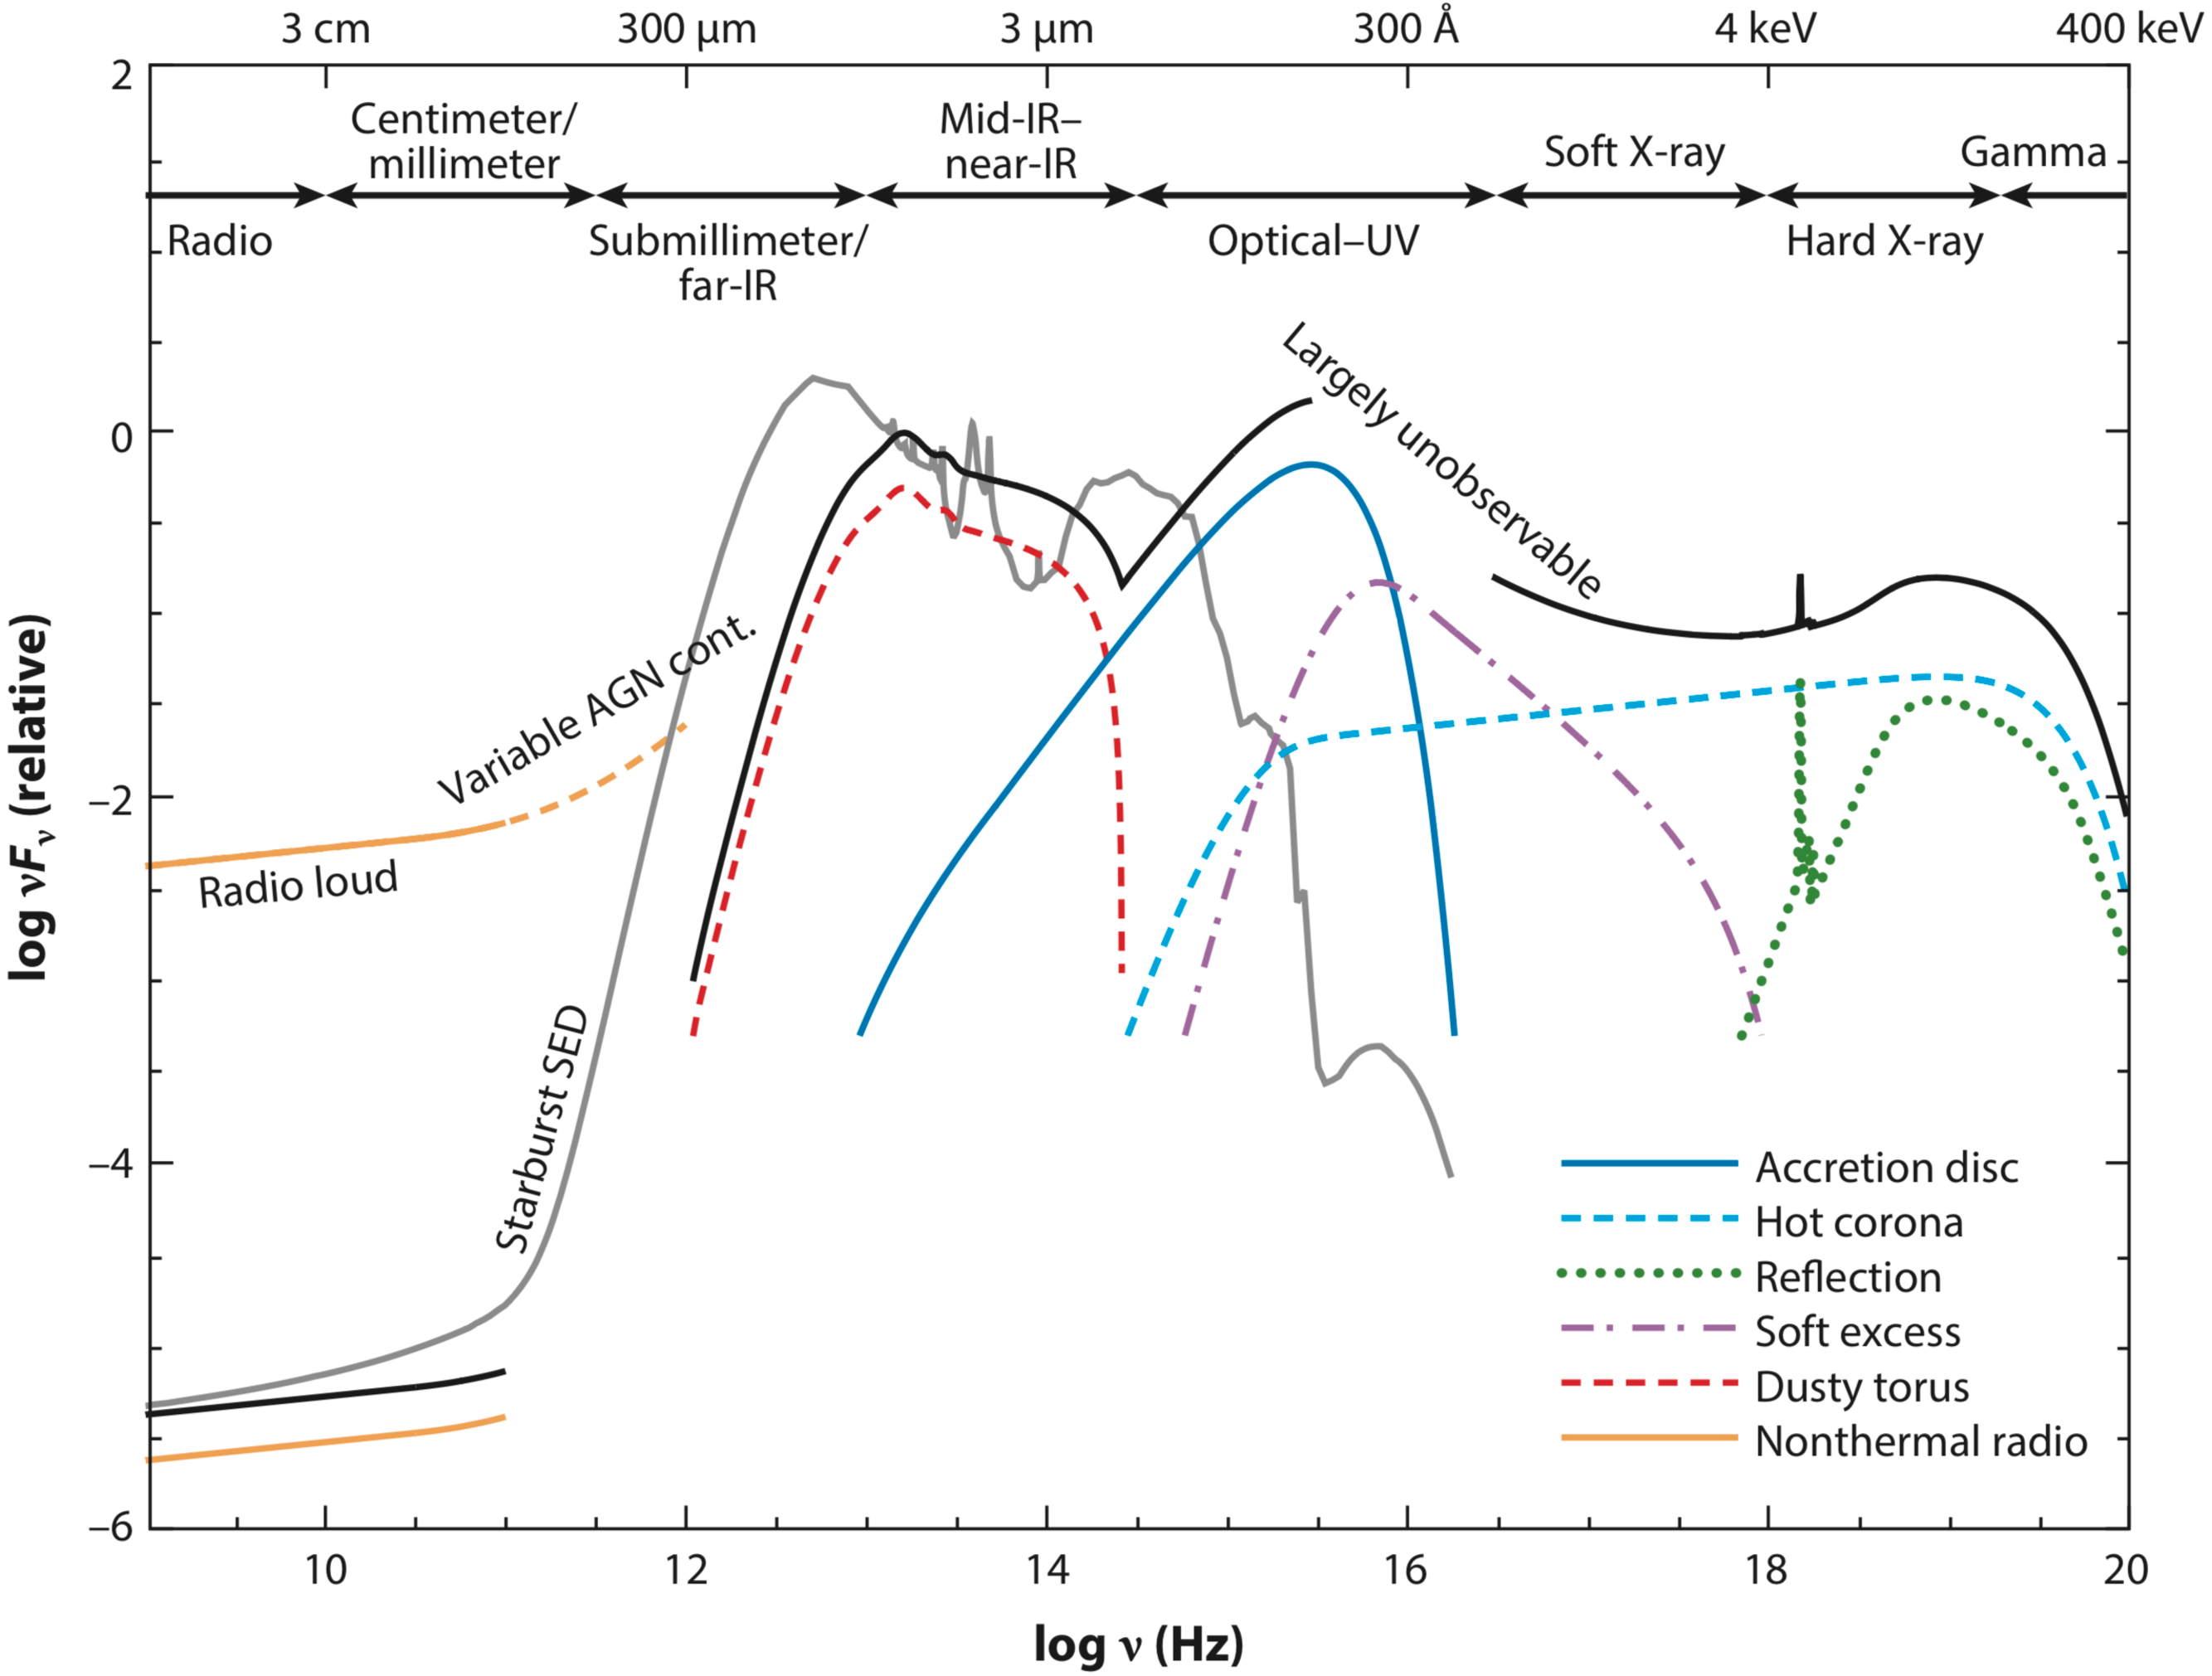
\includegraphics[width=\textwidth]{Figs/Intro/Fig1_Hickox18.pdf}
  \vspace{-30pt}
  \caption{Spectral energy distribution of an AGN. Figure from \citet{2018ARA&A..56..625H}}
    \label{fig:AGN_SED}
\end{center}
\end{figure}

The infalling gas will produce an optically thick disk of material, an accretion disk on a subparsec scale, that will emit thermally because of its own viscosity \citep[e.g.][]{1973A&A....24..337S, 1984ARA&A..22..471R}. The temperature of the gas will increase as it approaches the SMBH and in a typical AGN will range at $T \approx 10^3-10^4 K$ corresponding to a majority of the emission at $\approx 30-300 nm$ (blue line in Fig.~\ref{fig:AGN_SED}).
Around the accretion disk there is a geometrically and optically thick warm–hot dusty and molecular torus which is at a luminosity dependent distance, but within the gravitational influence of the SMBH. It may be considered as the extension of the accretion disk at a distance where dust and molecules can form. The torus is heated by the absorption of shorter-wavelength photons from the accretion disk which it will in turn then re-emit thermally at lower energies, at NIR and MIR wavelengths (red dashed line in Fig.~\ref{fig:AGN_SED}).
Another important source of emission from the black hole is a hot corona above the central part of the accretion disk. This emits in the X-rays through inverse Compton scattering of photons from the accretion disk with relativistic electrons and has a power law shape $N(\nu)\propto \nu^{-\Gamma}$, with $\Gamma=1.8\pm0.2$ (light blue dashed line in Fig.~\ref{fig:AGN_SED}). 
The relativistic electrons in the corona and also in large-scale radio jets can generate synchrotron radiation observable in the radio (yellow line in Fig.~\ref{fig:AGN_SED}).
The primary X-ray continuum can be reprocessed via Compton scattering and photoelectric absorption, thus leading to two important features in the X-ray spectrum: the \kalfa{} emission line and the so-called "Compton-hump", together known as the AGN "reflection" component (green dotted line in Fig.~\ref{fig:AGN_SED}).

In the optical bands, the observed spectrum strongly depends on the inclination of the object. If the dusty torus inclination allows to observe the inner regions we will see emission lines from the broad line region, which is a high density region at about 0.01-0.1pc from the SMBH, close to the accretion disk, where the gas reaches speeds of thousands of km/s. The narrow line region is more external, within the central kiloparsec \citep[e.g.][]{2015MNRAS.454.4452H,2016MNRAS.460..130V}, and is less dense, therefore allowing for forbidden line transitions with lower velocity dispersions, of a few 100s of km/s.

\section{The connection between SFR and BH accretion}
Observational studies and cosmological simulations have revealed a deep interconnection between galaxies and their central supermassive black hole (SMBH): they appear to coevolve and affect each other during their lives.
It has been reported several times that the SMBH mass (M$_{\rm BH}$) correlates with a number of galaxy properties, including bulge mass, stellar velocity dispersion, and starlight concentration as quantified for example by the S\'{e}rsic index. The existence of these relations is not trivial to explain since the SMBH has a very small sphere of influence compared to the galaxy size. While it is relatively easy to explain that gas inflows from the intergalactic medium can feed the star formation during secular processes, it is not easy to understand how the gas loses angular momentum and funnels to the center of the galaxy to feed the SMBH \citep{2019NatAs...3...48S}. %{\bf explicitar que estas relaciones no son obvias, el BH es demasiado pequeño para influenciar directamente la dinámica de la galaxia.} %The relation with the velocity dispersion appears to the most fundamental relation so far \citep[e.g.,][]{2007ApJ...660..267B, 2016MNRAS.460.3119S, 2017MNRAS.466.4029S,2019MNRAS.485.1278S}.
\citet{2007ApJ...660..267B} have seen that a selection effect caused samples of AGN galaxies to be biased to higher velocity dispersions $\sigma$ at a given optical or NIR luminosity $L$. By modeling this bias they were able to show
%By modeling the selection bias that leads to the M$_{\rm BH}$ and velocity dispersion $\sigma$ and M$_{\rm BH}$-galaxy bulge luminosity from optical or NIR bands $L$, \citet{2007ApJ...660..267B} have shown 
that the most fundamental relation is between M$_{\rm BH}-\sigma$ while the relation between M$_{\rm BH}- L$ is a consequence of a relation between $\sigma-L$ and is therefore more biased, as it overpredicts abundances of massive BHs. %{\bf poner un par de oraciones explicando qué es el bias y por qué importa. RC: No entiendo. Si algo està biased significa que està equivocado y para que esté lo màs correcto posible es importante minimizar los bias. Pero eso es algo que cada astrónomo/físico debería saber. A qué te refieres?} 
Also \citet{2017MNRAS.466.4029S} showed that M$_{\rm BH}-\sigma$ is the most fundamental in the scaling relations between black holes and galaxies by studying the residuals of the relations between M$_{\rm BH}$ and $\sigma$, S\'{e}rsic index $n$ and M$_{\rm bulge}$ in SDSS galaxies. Finally, Monte Carlo simulations have shown that a bias can be introduced when dynamically measuring M$_{\rm BH}$: the requirement that the black hole sphere of influence must be resolved to measure black hole masses leads to an increased M$_{\rm BH}-\sigma$ relation of at least a factor three \citep{2016MNRAS.460.3119S}.
%\citet{2007ApJ...660..267B} have modeled the selection bias that leads to the M$_{\rm BH}$ and velocity dispersion $\sigma$ and M$_{\rm BH}$-galaxy bulge luminosity $L$, from optical or NIR bands, and have shown that the most fundamental relation is between M$_{\rm BH}-\sigma$ while the relation between M$_{\rm BH}- L$ is a consequence of a relation between $\sigma-L$ and is therefore more biased, as it predicts more massive BHs at a given luminosity. 
%\citet{2016MNRAS.460.3119S} found through Monte Carlo simulations that a bias can be introduced when dynamically measuring M$_{\rm BH}$: the requirement that the black hole sphere of influence must be resolved to measure black hole masses leads to an increased M$_{\rm BH}-\sigma$ relation of at least a factor three. 
%\citet{2017MNRAS.466.4029S} lead a study in which they studied the residuals of the relations between M$_{\rm BH}$ and $\sigma$, S\'{e}rsic index $n$ and M$_{\rm bulge}$ in SDSS galaxies, and find that $\sigma$ is the most fundamental in the scaling relations between black holes and galaxies.

Interesting insight in this respect has been gained by studying the cosmic star formation rate density (SFRD) and black hole accretion rate densities (BHARD), which are the amount of star formation and black hole accretion per unit of comoving volume at a given redshift. With the fundamental contribution from deep and wide field surveys it has been possible to study them thoroughly and to unveil their evolution.
As can be seen in Fig.~\ref{fig:BHARD}, the BHARD has been determined from IR observations with \emph{Herschel} \citep{2010A&A...518L...1P} and from X-ray observations with XMM-Newton \citep{2001A&A...365L...1J} and Chandra \citep{2000SPIE.4012....2W}. In the IR it was possible to determine the BHARD up to $z\sim3$ \citep{2014MNRAS.439.2736D}, while in the X-rays, thanks to wide and deep surveys it was possible to determine it up to $z\sim 6$ \citep{2018MNRAS.473.2378V}.
%The BHARD has been determined from the IR (up to $z\sim3$, using and \emph{Herschel} data, \citet{2014MNRAS.439.2736D}) and X-ray observations (up to $z\sim 6$ wide and deep surveys from XMM-Newton and Chandra, \citet{2018MNRAS.473.2378V}). 
The history of star formation in galaxies throughout the life of the Universe has been thoroughly constrained in recent years: %it can be estimated from the UV emission of the massive and short-lived stars, but a fraction of it is absorbed by the dust present in the galaxy and then re-emitted in the IR, therefore the SFRD has been studied 
through infrared data with \emph{Herschel}, ultraviolet data with \emph{Galaxy Evolution Explorer} (GALEX) \citep[see][for a review]{2014ARA&A..52..415M} and more recently complemented by sub-mm ALMA data, especially at high redshift up to $z\sim10$ \citep{2020ApJ...902..112B,2020A&A...643A...8G}. %For both SFRD and BHARD the contribution from deep and wide field surveys has been of crucial importance. 
All of these studies have shown that both BHARD and SFRD reach a peak of activity at redshift $z\sim2$ and then decrease to the present epoch \citep{1998MNRAS.293L..49B}.

\begin{figure}
\begin{center}
  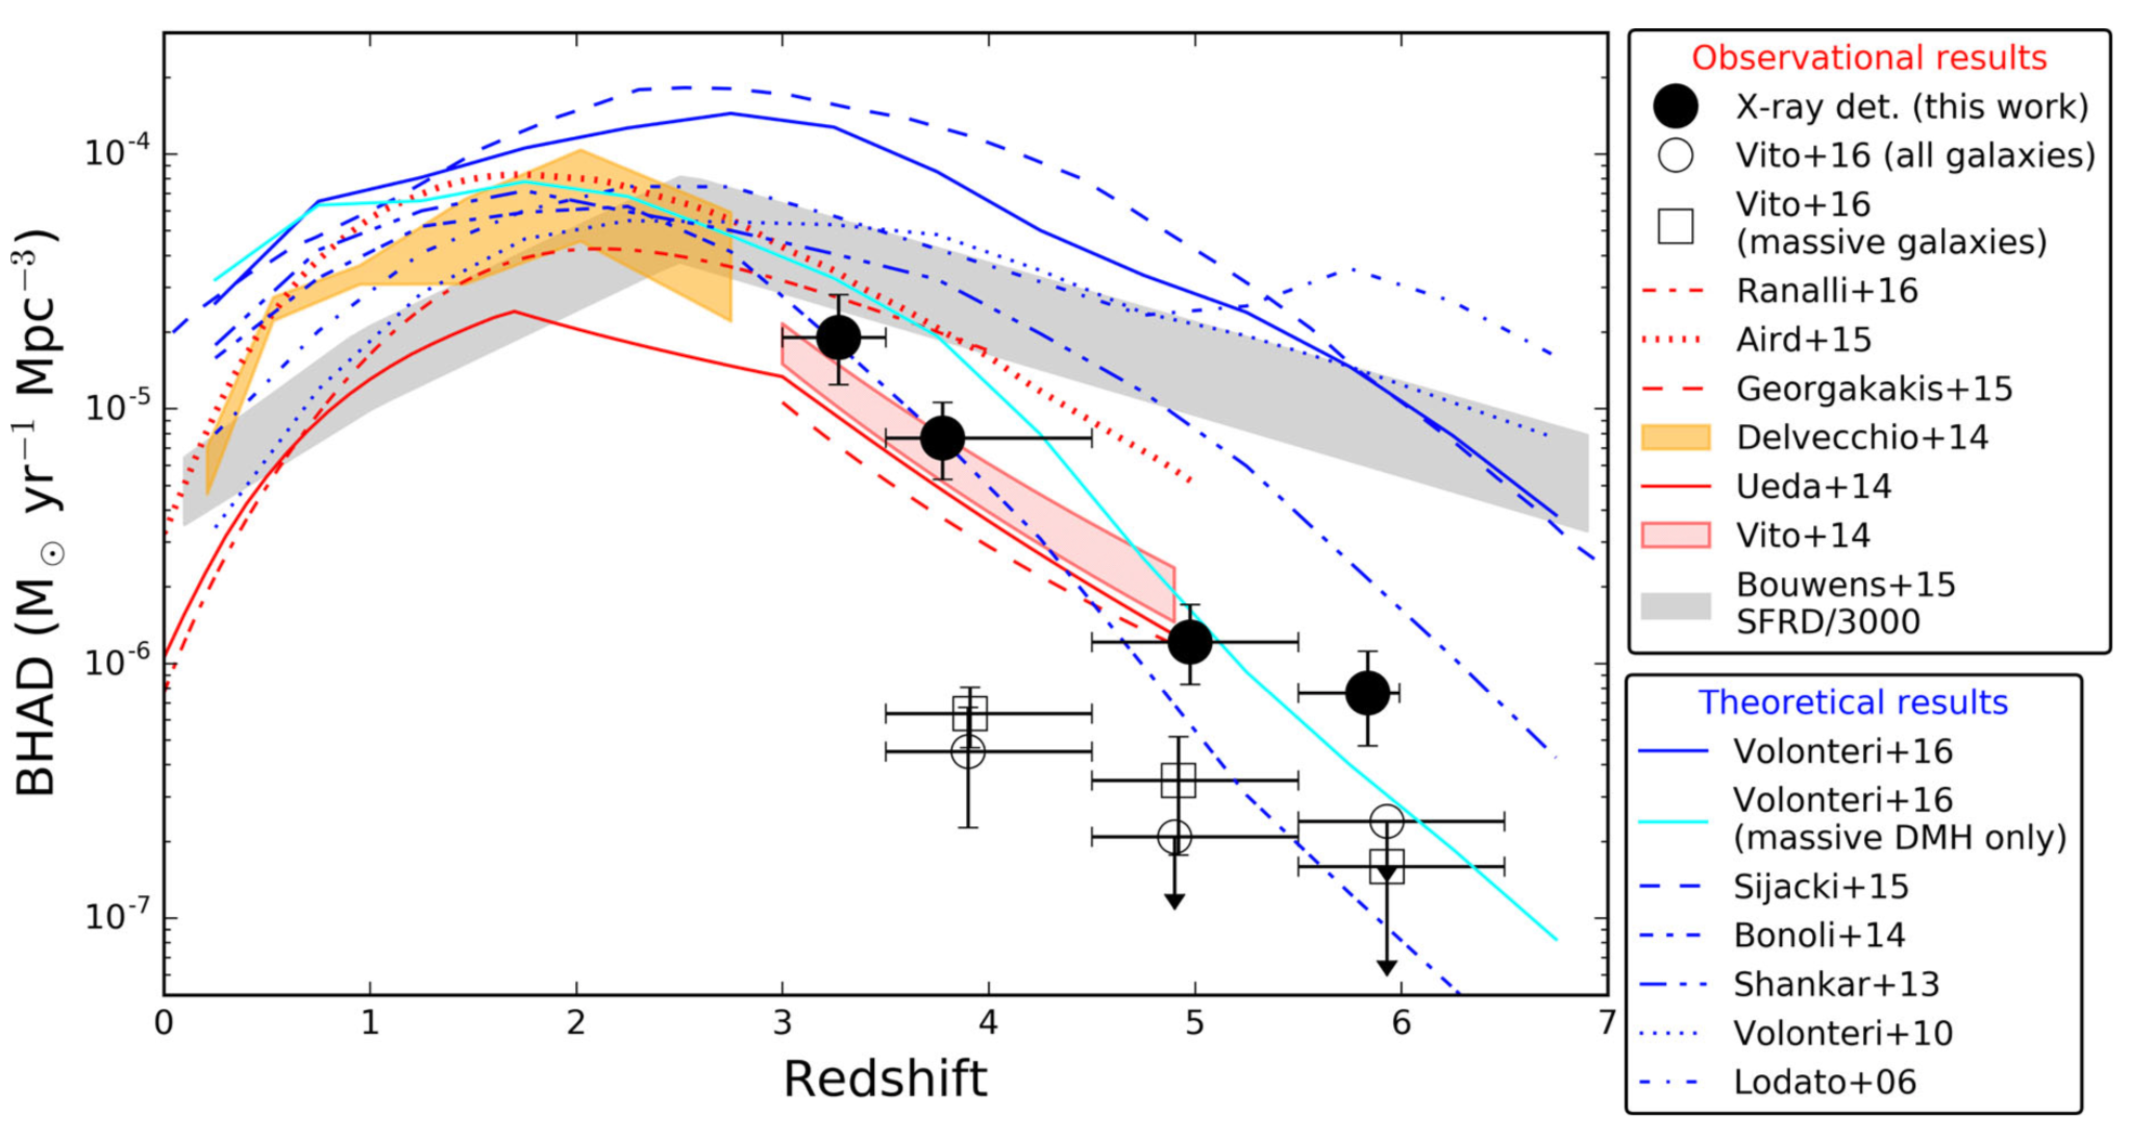
\includegraphics[width=\textwidth]{Figs/Intro/BHARD_Vito18.pdf}
  \vspace{-30pt}
  \caption{BHARD from \citet{2018MNRAS.473.2378V} and other works as reported in the legend. SFRD from \citet{2015ApJ...803...34B} is also reported for comparison purposes.}
    \label{fig:BHARD}
\end{center}
\end{figure}

Additionally, semianalytic models and hydrodynamic simulations show that a self-regulating mechanism, the so called feedback, is required between the star formation and the black hole accretion in order to reproduce local scaling relations, i.e. relations that describe strong trends that are observed between important physical properties of galaxies %{\bf definir scaling relations o al menos recordar lo de arriba y decir relacion entre BH mass y host galaxy properties.}
\citep[see][for a review]{2015ARA&A..53...51S}. Since the pioneering models of galaxy evolution in a cold dark matter framework it was clear that there was an ``overcooling problem'': most of the gas should have cooled and condensed into stars by the present day while it is observed that less than 10\% of it is in the shape of stars, so some suppression of cooling and star formation had to be introduced. This could be as energy released by supernovae \citep{1974MNRAS.169..229L,1978MNRAS.183..341W,1986ApJ...303...39D,1991ApJ...379...52W} and the impact of this phenomenon would be important in regulating star formation in low mass galaxies. On the other hand, luminosity functions predict more high luminosity galaxies in the local universe than we observe, and this might be prevented from happening through feedback from the SMBH as it actively accretes gas %, which is called an active galactic nucleus (AGN)
.%{\bf definir AGN y feedback}
 %AGN also emit in the X-rays, IR and in the radio. The X-ray emission is thought to originate in a corona above the accretion disk by inverse Compton scattering. The IR emission is reprocessed emission from torus and radio from non thermal bremsstrahlung.
The accretion of gas in the BH is an very efficient process, and a fraction of $\approx 5-45\%$, depending on the spin of the black hole \citep[e.g.][]{1963PhRvL..11..237K,1983bhwd.book.....S}, will be emitted as electromagnetic radiation, thereby allowing for very high AGN luminosities.
Simple calculations have shown that when the black hole becomes sufficiently massive ($> 10^7 M_\odot$) its maximum accretion luminosity, the Eddington %{\bf definir Eddington, o decir simplemente maximum accretion luminosity, definir accretion, en realidad, antes de hablar de esto poner qué es un AGN y por qué brilla y por qué podría afectar a su galaxia, ponle un parrafito sobre esto.}
luminosity, becomes high enough that its winds could in principle blow out all of the gas in the entire galaxy \citep{1998A&A...331L...1S}. This feedback mode, called quasar mode, prevents star formation by delivering momentum to the galactic gas and removing it. There is also a radio mode in which the BH is in a low accretion mode and heats the gas, thereby preventing it from collapsing and forming new stars \citep{2017NatAs...1E.165H}.
     
    The decline of the SFRD at low redshift is thought to depend on the decreasing availability of cold gas that is required to form stars and accrete onto black holes \citep[e.g.,][]{2016MNRAS.458L..14F}. Since most of the galaxies lie on the main-sequence of star-forming galaxies, they are the ones that dominate the SFRD evolution \citep{2011ApJ...739L..40R}. The observation of the main sequence at all redshifts and its lack of evolution of the slope, but only an increase of the normalization with redshift, reinforces the belief that most of the SF happens through secular processes \citep{2015A&A...581A..54T, 2015A&A...575A..74S, 2016ApJ...817..118T}: at earlier epochs, galaxies of a given stellar mass were forming more stars than in the local Universe.
    Starburst galaxies are instead a small fraction of star-forming galaxies that are undergoing a stochastic and short-lived episode of considerable galaxy growth, and their SFRs and gas fractions are higher than those on the MS at the same stellar mass, but they cannot be dominating the SFRD because of their low numbers \citep[$\sim2\%$][]{2011ApJ...739L..40R}. 
    Quiescent galaxies, on the other hand, have little star formation but have been shown to evolve from $z\sim1.8,$ where they have significant amounts of dust and gas ($\sim5-10\%$) but their star formation efficiency is low, to the local universe, where they are gas poor \citep{2018NatAs...2..239G}.
    
    Just like star formation, black hole accretion depends on the availability of cold gas. 
    In a classic evolutionary picture predicted by simulations one could have a star forming disk galaxy on the main sequence which undergoes a major merging event \citep{2005Natur.433..604D, 2008ApJS..175..356H}: During the early stages of galaxy merging, gas can efficiently cool and lose angular momentum, eventually feeding black hole growth and central star formation, producing a starburst. The black hole accretion is initially obscured by thick layers of dust, which are then possibly removed by its increasing radiation and momentum feedback, revealing the quasar. Eventually, the gas is consumed, the quasar luminosity fades rapidly, and the star formation episode ceases. This leaves a "red and dead" elliptical galaxy with no or very little star formation or black hole accretion \citep{2004ApJ...600..580G, 2006ApJ...650...42L}. This picture seems to be validated by low redshift (ultra) luminous IR galaxies ((U)LIRGs) which are starburst galaxies often undergoing a major merger event \citep{1996ARA&A..34..749S}, but it doesn't seem to apply to higher redshift galaxies, as many of these don't show signs of a disturbed morphology \citep{2007A&A...468...33E, 2019ApJ...877L..38R}. 
    
    Other theoretical models have predicted pictures of an in situ co-evolution scenario in which SF and black hole accretion are fed by the gas already present in the galaxy and triggered by the early collapse of the host dark matter halos  \citep[e.g.][]{2006ApJ...650...42L, 2011ApJ...742...24L, 2014ApJ...782...69L, 2013ApJ...772..119L,2015ApJ...810...74A, 2016ApJ...833..152M} and/or steady cold gas streams along filaments of the cosmic web  \citep[e.g.][]{2009Natur.457..451D, 2011ApJ...741L..33B}. The accretions are subsequently controlled by self-regulated baryonic physics and in particular by energy feedback from supernovae (SNe) and AGN. In this picture starbursts are gas rich young galaxies, placed to the left of the main sequence (as opposed to \textit{above}). These galaxies then evolve at about a constant SFR while increasing their stellar masses, thus reaching the main sequence locus \citep{2016ApJ...833..152M, 2018ApJ...857...22L}. Additionally \citet{2019MNRAS.482.4454W} find in their semi-analytic models of galaxy formation that not all galaxies in the starburst locus have recently undergone a major merger and that not all the galaxies which have undergone a major merger event result in a starburst.
    Observational results are still not capable to discern between these evolutionary scenarios as deep high resolution data for large statistical samples of starbursts are needed, and only future facilities will be capable to provide them. 
    
    These pictures might suggest that just like the majority of galaxies follow a main-sequence in the SFR-$M_*$ plane, a similar relation between the black hole accretion rate (BHAR) and the $M_*$ might exist: the more massive the galaxy, the higher the availability of inflowing gas for star formation and black hole accretion, which would mean that they both should correlate with stellar mass. In addition, galaxies offset from the main-sequence (starbursts and quiescents), might have a BHAR that varies accordingly with the gas that is typically available in that phase \citep{2019ApJ...877L..38R}. 
    
    In order to search for these potential correlations, many authors have used the X-ray luminosity of galaxies as a proxy of BHAR: X-rays are very energetic photons that are created very close to the central SMBH, and other contaminants in the host galaxies at these wavelengths, for example, emission from stellar processes or binary systems, are usually less powerful and not dominant \citep[e.g.][]{2015A&ARv..23....1B}. Nevertheless, the first studies that traced the instantaneous BHAR with X-ray flux failed at finding any BHAR-M$_*$ relation \citep{2009ApJ...696..396S, 2010A&A...518L..26S, 2012MNRAS.419...95M, 2012A&A...545A..45R, 2015ApJ...806..187A}. A lack of a correlation between SFR and BHAR does not by itself necessarily imply a lack of physical connection. It might arise, for example, from different duty cycles and variabilities that characterize the two processes.  
    Episodes of star formation last for several Gyr, while the SMBH duty cycles are believed to be very short, with accretion episodes of about $10^5$~yr and variability timescales that range from minutes to months.
    
    In order to constrain more robust and reliable BHAR, 
    it is thus necessary to average their growth rate over a long time interval. A very promising technique to achieve this goal consists of stacking X-ray images. Since the BHAR is a stochastic event, stacking large samples of galaxies in a given volume, by grouping them based on optical properties, e.g. the stellar mass,  is equivalent to averaging the growth rate of all galaxies.
    Furthermore stacking allows us to perform studies on mass-complete samples by averaging the count rates of the X-ray images in the optical positions of the galaxies, thus increasing the signal-to-noise ratio, and allowing us to reach fluxes well below the single-source detection threshold of the observations. %{\bf poner en otra oracion que el stacking se hace para galaxias con las mismas caracteristicas opticas, que quede claro que no se está mezclando todo} {\bf pondría esto último primero, que es lo esencial para calcular el crecimiento promedio}
    Previous works indeed searched for a relation between M$_*$ and average BHAR by stacking X-ray images \citep[e.g.,][]{2012ApJ...753L..30M, 2015ApJ...800L..10R, 2017ApJ...842...72Y}, and the probability distribution of specific X-ray luminosity (X-ray luminosity divided by galaxy stellar mass) %{\bf per galaxy? per bin?} 
    with a maximum likelihood approach \citep{2012ApJ...746...90A, 2012MNRAS.427.3103B, 2018MNRAS.475.1887Y} and a Bayesian approach \citep{2018MNRAS.474.1225A}. All studies point toward a positive correlation between the BHAR and the M$_*$ for star-forming galaxies, very similar to the main-sequence of star-forming galaxies, with a slope close to unity, non-negligible redshift evolution, a positive slope for the BHAR-to-SFR ratio as a function of stellar mass, and indications of different behaviors for quiescent and starburst galaxies. 
    Thus far, no study has presented a complete analysis throughout all galaxy life phases by highlighting the evolution of the accretions and the BHAR-to-SFR ratio throughout cosmic time. This is what we present here, in order to understand if the efficiencies of gas conversion in the black hole correspond to those of the star formation, how they vary with time, stellar mass and especially with galaxy life phase. %{\bf pon más explicitamente que interrogante se va a responder con este analisis más completo, aunque sea en varias oraciones. Hay teorías alternativas que se van a probar?} 
    So far, only \citet{2019MNRAS.484.4360A} have shown that the fraction of AGN galaxies is higher below the main-sequence and in starbursts than in the main sequence. %{\bf and SF's?, aquí veremos qué pasa en las otras fases? para restingir qué cosa?}.
        
        We here characterize the evolution of the average BHAR for normal star-forming, quiescent, and starburst galaxies at $0.1<z<3.5$. This redshift interval encompasses the majority of the history of the Universe and contains two crucial epochs in its evolution: the peak of the star formation rate density and BHAR of the Universe at z$\sim$2, and their decline to the local Universe. In Chapter~\ref{ch:observations} 
        we take advantage of the unique depth, area, and wavelength coverage of the COSMOS field, which allows us to select a mass-complete sample with large statistics out to very high redshifts for each galaxy phase. This is particularly important for starbursts, which are rare objects and require a large field in order to be found in good numbers for statistics.
        %We apply the stacking technique to X-ray images from the \textit{Chandra} COSMOS-Legacy survey \citep{2016ApJ...819...62C} and combine the results with the actual X-ray detections in order to estimate the average X-ray luminosity and therefore average BHAR. We compare the evolution of the average BHAR with that of the average SFR. We show that these data confirm and extend previous claims about the evolution of the specific accretions and that the ratio of BHAR to SFR and M$_*$ are correlated. 
        Then in Chapter~\ref{ch:SEM} we use the unique flexibility and simplicity of semi-empirical models to generate mock galaxy catalogs and perform an analogous analysis in order to explore the parameters that rule the relation between the ${\rm L}_{\rm X}$ (or BHAR) and stellar mass in galaxies across the same redshift range and evolutionary stages.
        
        \section{Gas in active galaxies in the local universe}
        On a different approach, in Chapter \ref{ch:gas_distribution} we study the distribution of the gas generating the X-ray reflected component (green dotted line in Fig.~\ref{fig:AGN_SED}) in a sample of local active galaxies, by assuming that the reflected emission comes from the X-ray continuum and is reprocessed by a dense layer of gas which will produce \kalfa{} emission and damp the variations of the continuum based on its size. We work with a sample of galaxies from Andonie et al. (in prep.) for which we have light curves of both the continuum and \kalfa{} line extracted from Chandra and XMM archival data. We run Monte Carlo simulations of these light curves, modeled as red noise, in order to determine the size of the reprocessing gas based on the observed smoothing of the \kalfa{} light curves.
